\chapter{Pair Interaction LGCA}
Pair-interaction automata (PI) constitute another branch that successfully evolved from HPP model, somewhat in contrast to FHP.
To put it in a nutshell, FHP changed the rectangular grid for hexagonal, and thus obtained better rotational symmetry, increased the degree of freedom of the nodes and added new collision states. 

The pair-interaction model preserves the HPP rectangular lattice, and the degrees of freedom in the node are incremented by the artificial definition of momentum.
%In FHP and HPP, momentum of the particle corresponds to its lattice velocity, or equivalently, to the cell that the particle occupies.
Momenta has no longer same direction as the lattice velocities, but they constitute another degree of freedom of the particle, that might change in the collision, independently of the lattice velocity. 
Although the differentiation in momentum and velocity might seem odd at the first glance, we will show that it leads to the physically correct microdynamics and offers us very efficient algorithm for implementation.

\bigskip
We will explore theory of Pair Interaction automaton in arbitrary dimension later on, but to get good understanding of the pair-interactions, we start with its $2$D version, so we can explain the theory graphically.

\section{User-friendly guide to Pair interactions}

\subsection{Pair-interactions automaton in two dimensions}

Geometry of the lattice is same as for HPP model. It consists of nodes arranged in the rectangular grid:

\begin{figure}[htbp]
 \centering 
 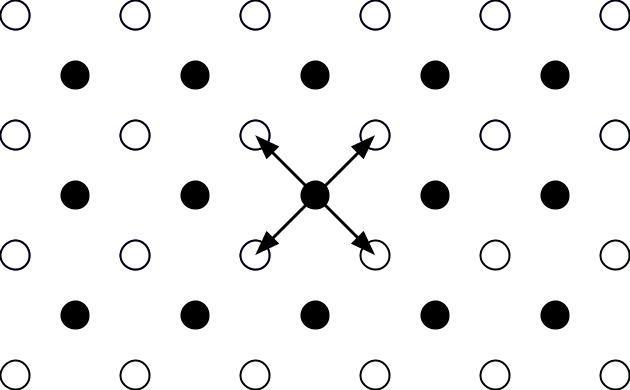
\includegraphics[width=0.9\textwidth]{./img/pi_grid}
 \label{2dgrid}
 \caption{Lattice of 2D Pair Interaction automaton}
\end{figure}

Every node (the cirlce on the picture above) is connected to 4 diagonal neighbors.
Let us consider this interesting 
If we look on the node in more detail, it looks like this:

\begin{figure}[htbp]
 \centering 
 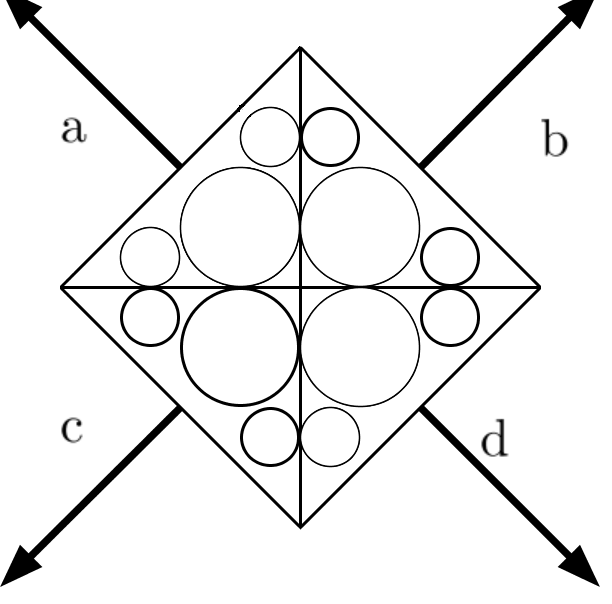
\includegraphics[width=0.3\textwidth]{./img/node_empty}
 \label{empty}
 \caption{A node in detail}
\end{figure}

\newpage
It consists of 4 cells ( \textbf{a,b,c,d} ) that are represented by 3 bits:
% on the picture. Each cell is represented by 3 bits:
one mass bit (a big circle) and two momentum bits (small circles).

The node on the picture above is empty (all bits are set to zero).

Here we have another example of a node:
\begin{figure}[htbp]
 \centering 
 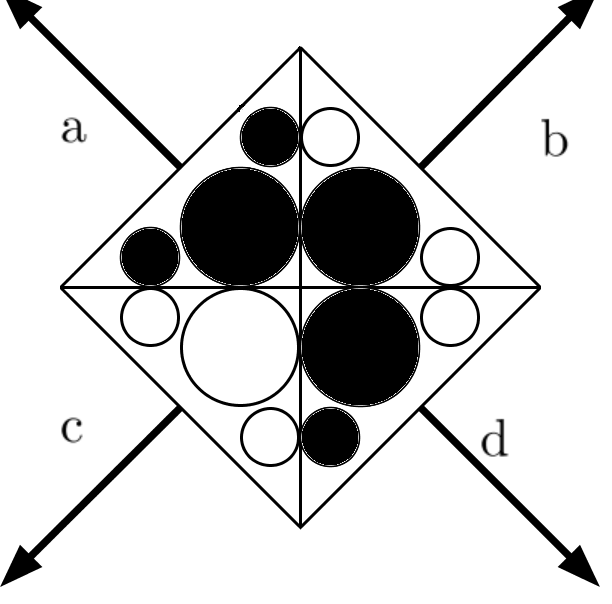
\includegraphics[width=0.5\textwidth]{./img/node_1}
 \label{pre_collision}
 \caption{State of a node before collision}
\end{figure}

In this node, there are particles in the cells a,b,d (mass bit is set to 1 - the big circle is black).

Particle in the cell \textbf{a} is standing (both momentum bits are 0).

Particle in the cell \textbf{b} has momentum in direction [1,1] and particle in the cell \textbf{d} has momentum in direction [0,1].

\subsection{Update rules}
Following rules are true of every lattice-gas cellular automaton.

\begin{enumerate}
\item Lattice is changing in discrete time steps
\item Update rules are \textbf{local}. It means that state of the cell in the next step is determined by the current state of the cell itself and its four neighbors. Hence we can resolve update of the lattice node by node (suitable for parallel computing)
\item If this cellular automaton really simulates fluid dynamics and is physically realistic, update rule needs to conserve \textbf{mass, momentum and angular momentum}.
\end{enumerate}

Update of the lattice is done in two steps, collision and propagation.


\subsection{Collision}
Collision changes configuration inside the single nodes. We require that momentum and mass is preserved in this step.

1) First, the cells are paired in X direction:
\begin{figure}[htbp]
 \centering 
 \includegraphics[width=0.3\textwidth]{../obrazky/x-interaction}
 \label{xinter}
 \caption{Pairs in X-direction}
\end{figure}

Then we swap the bits in the pairs so that total momentum in the pair is preserved. Therefore, node in \ref{pre_collision} changes to

\begin{figure}[H]
 \centering 
 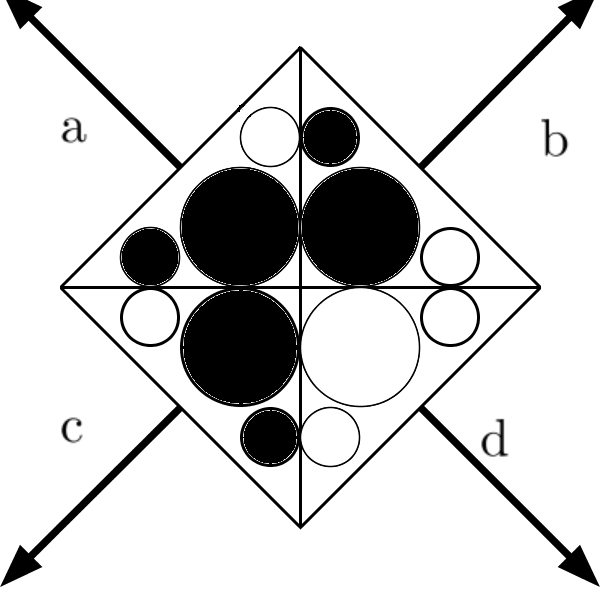
\includegraphics[width=0.5\textwidth]{./img/node_2}
 \label{colision1}
 \caption{State of the node after pair-interaction in X direction}
\end{figure}

2) Then, the cells are paired in Y direction:
\begin{figure}[htbp]
 \centering 
 \includegraphics[width=0.3\textwidth]{../obrazky/y-interaction}
 \label{yinter}
 \caption{Pairs in Y-direction}
\end{figure}

 Then we change the configuration in these pairs preserving mass and momentum in the node. Hence, the node in \ref{colision1} changes into:
 \begin{figure}[htbp]
 \centering 
 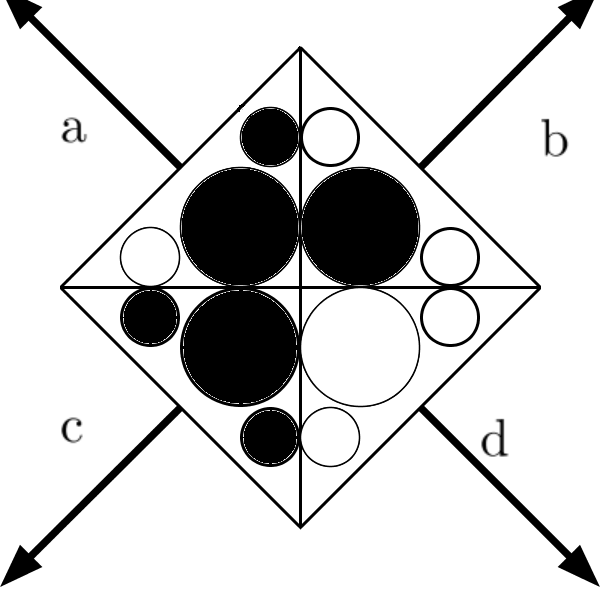
\includegraphics[width=0.5\textwidth]{./img/node_3}
 \label{colision2}
 \caption{State of the node after pair-interaction in Y-direction}
\end{figure}
\newpage
Actually, there is only 17 different configurations of the pairs. So instead of computing new configuration during every pair-interaction, we can just look in the table \ref{transitions} below and change the configuration accordingly. We consider this to be the greatest practical advantage of PI comparing to other methods.
\newpage
\begin{figure}[htbp]
 \centering 
 \includegraphics[width=0.7\textwidth]{../obrazky/transitions}
 \label{transitions}
 \caption{All admissible pair-interactions}
\end{figure}

\section{Propagation:}
Particles propagates from a single node to the four neighboring nodes along the lattice vectors, see \ref{2dgrid}.

Particle from the cell \textbf{a} propagates to the node up-right, to the cell \textbf{a} as well.

Analogously, particle from cell \textbf{b} propagates to the node up-left, to the cell \textbf{b}.

Of course, particle carries all its bits (its momentum).



Generalization of this automaton to arbitrary dimension D is very straight-forward. But we need to establish some mathematical formalism, as we haven't learned to draw D-dimensional pictures.

\section{3D Pair-interaction cellular automaton}

\begin{center}
    \begin{tabular}{| l | l | l | l |}
    \hline
    \multicolumn{3}{|c|}{DIFFERENCES BETWEEN \textbf{2}D AND \textbf{N}D PAIR INTERACTION}\\ \hline
     & \textbf{2dim PI CA} & \textbf{Ndim PI CA} \\ \hline
    \textbf{nodes} & $4$ cells arranged into square & $2^D$ cells arranged in hypercube \\ \hline
    \textbf{cells} & 1 mass bit, 2 momentum bits  & 1 mass bit, N momentum bits \\ \hline
    \textbf{neighbors} & node has 4 neighbors & node has $2^D$ neighbors  \\ \hline
    \end{tabular}
\end{center}

In his famous paper, Nasilowski defined and used formalism that:
\begin{enumerate}
\item is more difficult then is necessary in our opinion (and in few cases he redefines it along the way)
\item therefore his arguments are more difficult then necessary
\end{enumerate}


Instead, we will stick to the more modern formalism that we have been using.
We consider it more brief and effective and reader should be already familiar with it.

In previous chapter, reader should get good understanding how 2D Pair-interaction works.
believe that reader has already good idea how 2D Pair-interaction automaton works.

State of the node will be denoted by $\bm{n}(t,\bm{r})$, where $\bm{r}$ is its position on the lattice and $t$ is the current time step. $\bm{n}(t,.)$ represents the whole lattice at time $t$, sometimes we can the time variable and use only $\bm{n}(.)$.

Each node consists of $2^D$ cells:
\begin{equation}
\bm{n} = (n_1, n_2, ... , n_{2^D})
\end{equation}
State of each node is given by $2^D(D+1)$ bits: 
\begin{equation}
\bm{n} = \big\{ n_{i\alpha} \in \big\{0,1\big\},~i = 1..2^D, ~\alpha = 0,1,...D\big\}
\end{equation}
where index $i$ specifies cell of the node, and index $\alpha$ specifies the momentum bit of the cell. Actually, they are the Cartesian coordinates of the cell momenta.



Evolution of the lattice happens in discrete time steps - updates $\mathcal{U}$:

\begin{equation}
\mathcal{U} \bm{n}(t,.) = \bm{n}(t+1,.)
\end{equation} 
Update operator $\mathcal{U}$ can be further divided in two operations, collision $\mathcal{C}$ and propagation $\mathcal{P}$:
\begin{equation}
\mathcal{U} = \mathcal{P} \circ \mathcal{C}
\end{equation} 

\section{Collision}

The purpose of collision is to change the state of the node $\bm{n}$ into new state $\bm{n'}$ such that 2 conditions are fulfilled:

\begin{enumerate}
\item \textbf{Collision operator is one-to-one}:

If $\mathcal{C}: \bm{n} \rightarrow \bm{n'}$,
then $\mathcal{C}: \bm{n'} \rightarrow \bm{n}$.

This reversibility condition allows us to apply Gibbs formalism later on.

\item \textbf{Collision preserves mass and momentum in the nodes}

Mass and momentum are given by
\begin{equation}
m_0 = \sum_i n_{i0}
\end{equation}
\begin{equation}
p_{\alpha} = \sum_i c_{i\alpha} n_{i\alpha},~\alpha=1,2,...D
\end{equation}

Using these definitions, condition of mass and momentum conservation could be expressed by:
\begin{align}\label{mmc}
\begin{split} 
m_o = m'_o &~~ \Leftrightarrow ~~ \sum_i n_{i0} = \sum_i n'_{i0}, \\
p_{\alpha} = p'_{\alpha} &~~ \Leftrightarrow ~~ \sum_i c_{i\alpha} n_{i\alpha} = \sum_i c_{i\alpha} n'_{i\alpha}, ~\alpha=1,2,... D 
\end{split}
\end{align}
\end{enumerate}


The easiest collision rule fulfilling these conditions would be identity
\begin{equation}
\mathcal{I}:\bm{n} \rightarrow \bm{n}
\end{equation}
but this "non-collision" would lead to undesired, non-physical invariants.
On the contrary, we want to change as many bits in the node as possible,
or to say it physically, change directions to as many particles as conservation of momentum allows.
Providing that, the mean free path of particles is reduced to minimum, and we can reach higher Reynold numbers in the simulations.

Such collision algorithm is surprisingly simple and was described in previous section graphically.
Now we state collision rule more formally for arbitrary dimension D.
The algorithm consists of D steps.
In each step ($d=1...D$), we create pairs of cells in $d^{th}$ direction, or equivalently, we create pairs $(n_i,n_j)$, such that $c_{id} = -c_{jd}$ and $c_{i\alpha} = c_{j\alpha}$ for $\alpha \neq d$.
If $n_{id} = n_{jd}$ (it means that in direction $d$, momentum of the pair is zero), we swap the states of the cells $n_i$ and $n_j$ without changing the total momentum of the pairs.
In the end of the collision, the total momentum of the node is conserved, because all the pair-interactions conserved the momentum.

\bigskip

%Parameters $\mu_{\alpha}$ are intensive thermodynamical parameters corresponding to the the extensive dynamical invariants $m_{\alpha}$.

\section{Equilibrium statistics}
We start by revoking the basic result of the microdynamics
\begin{equation} \label{over2}
\bm{n}(t+2,.) = \mathcal{U}^2 \bm{n}(t,.)
\end{equation}

In the odd and even time steps, the different parts of the hlattice are occupied, so it does not make sense to compare them.
That is why we are comparing states of the lattice over the two time steps.

The microdynamical equation \ref{over2} implies conservation of probabilities
\begin{equation} \label{cp}
P(t,\bm{n}(.)) = P(t+2,\mathcal{U}^2\bm{n}(.))
\end{equation}
where $P(t,n(.))$ is the probability of occurrence of lattice in some state $n(.)$ from the statistical ensable of automata.

\subsection{Gibbs distribution}

Let's see if the Gibbs probability distribution fulfill the conservation law \ref{cp}.

First we define the total momentum of the whole lattice $\mathcal{L}$:
\begin{equation} \label{momentum}
m_{\alpha}(.) = \sum_{i,\bm{r}} c_{i\alpha} n_{i\alpha}(\bm{r}),~\alpha=0,1,..D
\end{equation}

Now we can define Gibbs probability for our model:
\begin{equation}
P^E(n(.)) = \frac{W(n(.))}{Z}
\end{equation}
where
\begin{equation}
W(n(.)) = exp(-\sum_{\alpha = 0}^D \mu_{\alpha} m_{\alpha}(.))
\end{equation} 
and $Z$ is the partition function
\begin{equation}
Z = \sum_{n(.))} W(n(.))
\end{equation}

Conservation of local momenta \ref{mmc} implies conservation of the total momentum
\begin{equation}
m_{\alpha}(.) = m'_{\alpha}(.),~\alpha=0,1,..D
\end{equation}
that immediately implies conservation of Gibbs probability
\begin{equation}
P^E(t+2,\mathcal{E}^2n(.)) = P^E(t,n(.)).
\end{equation}

Additivity of the momentum cell by cell over the whole lattice (equation \ref{momentum}) implies that there is no statistical correlation between different cells:
\begin{equation}
P^E(n(.)) = \prod_{i,\bm{r}} P^E(n_i(\bm{r}))
\end{equation} 
Even further, if we consider, that
\begin{equation}
P(n_i(\bm{r})) = \frac{W(n_i(\bm{r}))}{Z}
\end{equation}
where
\begin{equation}
W(n_i(\bm{r}))=exp(-\sum_{\alpha = 0}^D\mu_{\alpha}c_{i\alpha}n_{i\alpha}(\bm{r})) = \prod_{\alpha=0}^Dexp(-\mu_{\alpha}c_{i\alpha}n_{i\alpha}(\bm{r})) = \prod_{\alpha = 0}^D W(n_{i\alpha}(\bm{r}))
\end{equation}
we can see that bits of the cells $n_{i\alpha},~\alpha = 1,2,...D$ are not statistically correlated.

For sure, they are correlated with $n_{i0}$, because $n_{i0} = 0 \Rightarrow n_{i\alpha} = 0~ for~ \forall ~ \alpha = 1,2,...D$.

But for $\alpha=1,2,...D$ we can write:
\begin{equation} \label{form2}
\sigma_{i\alpha} = prob(n_{i\alpha} = 1 | n_{i0} = 1) = \frac{W(n_{i\alpha})}{Z_{i\alpha}}
\end{equation}
where
\begin{equation}
W(n_{i\alpha}) = exp(-\mu_{\alpha}c_{i\alpha}n_{i\alpha})
\end{equation}
and
\begin{equation}
Z_{i\alpha} = \sum_{n_{i\alpha}=0}^1 W(n_{i\alpha}). 
\end{equation}
Hence
%\begin{align}
%\frac{1}{1 + \exp(\mu_{\alpha} c_{i\alpha})} := f(\mu_{\alpha} c_{i\alpha}).
%\end{align}

Little more laborious calculation would lead us to mean occupation numbers
\begin{equation} \label{form1}
\rho_i := <n_{i0}> = \frac{Z_i - 1}{Z_i} = \frac{e^{-\mu_0}\prod_{\alpha = 1}^D(1+e^{-{\mu_{\alpha} c_{i\alpha}}})}{1+e^{-\mu_0}\prod_{\alpha = 1}^D(1+e^{-{\mu_{\alpha} c_{i\alpha}}}) } = f\big(\mu_0 + \sum_{j=1}^d ln f(-\mu_j v_j) \big).
\end{equation}
$\rho_i$ can be interpreted as probability that cell $n_i$ is occupied, but also as the equilibrium mass of the cell.

To define the density, we need to consider what is the volume of the node. Since lattice vectors $c_{i\alpha}$ span interval $[-1,1]^D$, we can define volume V as
\begin{equation}
V = 2^D
\end{equation}
Then the mass density reads
\begin{equation}
\rho = 2^{-D} \sum_i \rho_i
\end{equation}
and the momentum density
\begin{equation}
q_a := 2^{-D} \sum_i c_{i\alpha} <n_{i\alpha}> = 2^{-D} \sum_i c_{i\alpha} \rho_i \sigma_{i\alpha}.
\end{equation}
It is efficient to use only one quantity instead of mass and momentum density, and our formalism invites us to do so. We define the \textbf{hypermomentum} density
\begin{equation} \label{hypermom}
q_{\alpha} := 2^{-D} \sum_i c_{i\alpha} <n_{i\alpha}>
\end{equation}
where $q_0$ is the mass density $\rho$, and $(q_1,q_2,...q_D)$ is the momentum density.

Expanding formulas \ref{form1} and \ref{form2} in Taylor series and inserting to the last equation leads to rather lengthy calculation (Appendix B in [2]), that results in 
\begin{align}
\begin{split}
\rho_i &= \rho + 2 \frac{1-\rho}{2-\rho} \bm{v}.\bm{q} + 2 \, \frac{(1-\rho)(1-2\rho}{(2-\rho)^2 \rho} \, \big[(\bm{v}.\bm{q})^2 - q^2 \big] + O(q^3), \\
\sigma_{ij} &= \frac{1}{2} + \frac{v_j q_j}{(2-\rho)\rho} + O(q^3)
\end{split}
\end{align}
%for $|\bm{q}| \ll 1$.

\section{Hydrodynamic description}
It is based on the assumption that the state of the cellular automaton is near its equilibrium.
In that case, the whole state of the automaton can be specified by a few macroscopic order parameters $q_{\alpha}$.

\bigskip

For example, expectation values $p_{i\alpha}$ are continuous differentiable functions of the parameter q
\begin{equation}
p_{i\alpha} = p_{i\alpha}(q, \nabla q, \nabla^2 q,...)
\end{equation}
and we can expand them in Chapman-Enskog series in terms of $p_{i\alpha}^{eq}$
\begin{equation} \label{expro}
p_{i\alpha} = p_{i\alpha}^{eq} + r_{i\alpha} + \mathcal{O}(\nabla^2)
\end{equation}
with
\begin{align}
r_{i\alpha} = \sum_{\beta j} R_{i\alpha \beta j } \nabla_j q_{\beta}.
\end{align}
We will use this expansion later on.

\bigskip

The resulting equations of this section will be the hydrodynamic equations for the pair-interaction automaton.

They are the set of evolution equations for the order parameters
\begin{equation} \label{evol}
\partial_t q_{\alpha} = \dot{q_{\alpha}}(q,\nabla q, \nabla^2 q,...)
\end{equation}
Due to conservation of the hypermomentum, the right hand side of \ref{evol} must be of the form
\begin{equation}
\dot{q_{\alpha}} = -\sum_k \nabla_k Q_{\alpha k}(q, \nabla q, \nabla^2 q).
\end{equation}

Let us look back to the microdynamical propagation equation
\begin{equation}
n_{i\alpha}(t+1,\bm{r} + \bm{c_i}) = n'_{i\alpha}(t, \bm{r}),
\end{equation}
that directly implies
\begin{equation} \label{micprob}
p_{i\alpha}(t+1, \bm{r} + \bm{c_i}) = p'_{i\alpha}(t, \bm{r}).
\end{equation}
If we expand $p_{i\alpha}(t+1, \bm{r} + \bm{c_i})$ in terms of $p_{i\alpha}(t,\bm{r})$, insert it to \ref{micprob} and apply $2^{-D}\sum_i c_{i\alpha}$ on both sides, we get
\begin{equation} \label{dens}
2^{-D} \sum_i c_{i\alpha} \big[(\partial_t + c_{i\alpha}\nabla_{\alpha}) + \frac{1}{2}(\partial_t + c_{i\alpha}\nabla_{\alpha})^2 + ... \big] p_{i\alpha} = 0
\end{equation}
The right-hand side disappeared because of the conservation of hypermomentum
\begin{equation}
2^{-D} \sum_i c_{i\alpha} p_{i\alpha} = 2^{-D} \sum_i c_{i\alpha} p'_{i\alpha}.
\end{equation}


Analogously to FHP and FCHC model, we can define various temporal and spatial scales (see Table \ref{scalings}) and expand operator of time derivative and space derivative into modes
\begin{equation} \label{exoper}
\begin{split}
\partial_t = \epsilon \partial_t^{(1)} + \epsilon^2 \partial_t^{(2)} + ...\\
\partial_{\alpha} = \epsilon \partial_{\alpha}^{(1)}
\end{split}
\end{equation}

Inserting \ref{expro} and \ref{exoper} into \ref{dens} leads to
\begin{equation}
\begin{split}
0 = 2^{-D} \sum_i c_{i\alpha}(\epsilon\partial_{t}^{(1)} + c_i \nabla_i) p_{i\alpha}^{eq} \\
+ 2^{-D} \sum_i c_{i\alpha}\big[\epsilon^2 \partial_t^{(2)} p_{i\alpha}^{eq} + \frac{1}{2}(\epsilon \partial_t^{(1)} + c_{i\alpha} \nabla_{\alpha})^2 p_{i\alpha}^{eq} \\
+ (\partial_t^{(1)} + c_{i\alpha} \nabla_{\alpha})\sum_{j \beta} R_{\beta j \alpha i}\nabla_{j}q_{\beta} \big] + \mathcal{O}(\nabla^3)
\end{split}
\end{equation}

Each order of $\epsilon$ must vanish separately.

For the terms linear in $\epsilon$ we get
\begin{equation}
2^{-D} \sum_i c_{i\alpha}(\partial_{t}^{(1)} + c_{i\alpha} \nabla_{\alpha}) p_{i\alpha}^{eq} = 0
\end{equation} \label{hydym}
or equivalently in terms of momentum density:
\begin{equation}
\partial_t^{(1)} q_{\alpha} + \sum_k \nabla_k Q_{\alpha k}^0 = 0
\end{equation}
where we used definition of hypermomentum \ref{hypermom},
and defined zero$^{th}$ term of momentum flux tensor $Q_{\alpha k}^0$:
\begin{equation}
Q_{\alpha k}^0 := 2^{-D} \sum_i c_{i\alpha}c_{i k} p_{i\alpha}^{eq}
\end{equation}

We can split equation \ref{hydym} into two -  mass density conservation and momentum conservation:
\begin{equation} \label{hyd1}
\partial_t \rho + \bm{\nabla . g^0}(\rho, \bm{q}) = \mathcal{O}(\nabla^2)
\end{equation}
\begin{equation}
\partial_t q_j + \sum_k \nabla_kQ_{jk}^0(\rho, \bm{q}) = \mathcal{O}(\nabla^2)
\end{equation}
where we used $g_k := Q_{0k}$.

\section{Hydrodynamic limiting cases}
In this section, we will derive hydrodynamic limiting cases of our model, that corresponds to four physical approximations,
namely
\begin{enumerate}
\item compressible Euler equation,
\item acoustic  limit,
\item inviscid incompressible Euler equation,
\item incompressible Euler equation with viscosity.
\end{enumerate}

Starting with equation \ref{hyd1}, blabla dokonci

expand in $\epsilon \ll 1$, that is defined as the Knudsen number (ratio  of mean free path and macroscopic scale).

\bigskip

\textbf{1) Compressible Euler equation}

For physical fluid, the equations read
\begin{align}
\begin{split}
\pd_t \rho + \bm{\nabla . q} = 0, \\
\pd_t q_j + \sum_k \nabla_k \big[ p(\rho) \, \delta_{jk} + \frac{1}{\rho} \, q_j \, q_k = 0
\end{split}
\end{align}

For our model, we need to pick up terms of order
\begin{align}
\begin{split}
\pd_t = O(\epsilon^2), ~ \bm{\nabla} = O(\epsilon^2),~\rho = \frac{1}{2} + O(\epsilon), \bm{q} = O(\epsilon) 
\end{split}
\end{align}
and we get

\begin{align}
\begin{split} \label{O2}
\pd_t \rho + \bm{\nabla.} \big[ \big( \frac{10}{9} - \frac{8}{9} big) \bm{q} \big] &= 0,\\
\pd_t q_j + \sum_k \nabla_k \big[\frac{\rho}{2} \delta_{jk} + \frac{8}{9}q_j\,q_k \big] &= 0
\end{split}
\end{align}

As in case of FHP, the absence of Galilei invariance in our model caused the unphysical dependence of the pressure $p$ on $\rho$.

\bigskip

\textbf{2) Acoustic limit}

Picking up the terms of order
\begin{align}
\pd_t = O(\epsilon),~ \bm{\nabla} = O(\epsilon),~ \rho = \rho_0 + O(\epsilon),~ \bm{q} = O(\epsilon)
\end{align}
leads to linear equations of sound
\begin{align}
\begin{split}
\pd_t \rho + 2\frac{1-\rho_0}{2-\rho_0} \bm{\nabla . q} = 0, \\
\pd_t \bm{q} + \frac{1}{2} \nabla \rho = 0 \,.
\end{split}
\end{align}



\textbf{3) Inviscid incompressible Euler equations}

For the ideal physical fluid (ideal fluid means inviscid and incompressible), the equations read
\begin{align} \label{ideal_phys}
\begin{split}
\bm{\nabla . u} &= 0, \\
(\pd_t + \bm{u.\nabla})\bm{u} + \nabla \Phi &= 0,
\end{split}
\end{align}
with $\Phi = p / \rho_0 = 2 p$ being the kinematic pressure.

For our model, taking terms of order
\begin{align}
\pd_t = O(\epsilon^3), \qquad \bm{\nabla} = O(\epsilon^2), \qquad \rho = \frac{1}{2} + O(\epsilon^2), \qquad \bm{q} = O(\epsilon)
\end{align}
from the expansion (cislo) leads us to
\begin{align}
\begin{split}
\bm{\nabla . q} &= 0, \\ 
(\pd_t + \frac{8}{9}\bm{q.\nabla})\bm{q} + \frac{1}{2} \bm{\nabla} \rho &= 0.
\end{split}
\end{align}

At last, our automaton got the hydrodynamic equations right, as we can easily transform then into \ref{ideal_phys} by setting
\begin{align} \label{transfor}
 \Phi = \frac{4}{9} \rho, \qquad \bm{u} = \frac{8}{9} \bm{q}.
\end{align}  
The $\bm{u}$ is the hydrodynamic velocity and 

Notice that the hydrodynamic velocity $\bm{u}$ is the momentum convection velocity, and can not be interpreted as the mean velocity of particles
\begin{align}
\bm{w} = \frac{\langle \sum_i v_i n_{i0} \rangle}{\langle \sum_i n_{i0} \rangle} = ... = \frac{2(1-\rho)}{(2 - \rho) \rho}\bm{q}.
\end{align}

The reason behind this difference lies in the broken Galilean invariance of our model.
The ratio between the velocities is called the "g-factor" ($g(\rho$), and for our special case, it is equal to
\begin{align}
\bm{w} = \frac{4}{3} \bm{q} = \frac{2}{3} \bm{u}.
\end{align}

It already arised in the FHP and FCHC model (where $g(\rho) \sim 1/2$ for small $\rho$).

\bigskip

\textbf{The Navier-Stokes equations}

For most applications, the inviscid incompressible approximation is too much idealized,
and we would like to find an approximation of Navier-Stokes equations
\begin{align} \label{nst}
\begin{split}
\bm{\nabla . u} = 0, \\
(\pd_t + \bm{u.\nabla}\bm{u} + \nabla \Phi = \nu \nabla^2 \bm{u}
\end{split}
\end{align}
with the friction term on the right hand side, containing the shear viscosity $\nu$.

For our model, the analogous set of equations is obtained by picking up terms
\begin{align}
\pd_t = O(\epsilon^2), \qquad \nabla = O(\epsilon), \qquad, \rho = \frac{1}{2} + O(\epsilon), \qquad \bm{q} = O(\epsilon).
\end{align} 
that leads to
\begin{align}
\begin{split}
\bm{\nabla . q} &= 0,\\ 
(\pd_t + \frac{8}{9} \bm{q . \nabla}) q_j + \frac{1}{2}\nabla_j\rho &= \sum_{klm} T_{jklm}\nabla_l \nabla_m q_k.
\end{split}
\end{align}

Is this set of equations equivalent to Navier-Stokes \ref{nst}?
If we could show that $T_{jklm}$ is isotropic, the equations would be equivalent by the transformation \ref{transfor}.
However, this is not the case, our model do not posses symmetries that forces $T_{jklm}$ to be isotropic.
We need to go to the second approximation to get more information of the tensor $T_{jklm}$.

Lengthy calculation that can be found in \cite{nasilowski} leads to
\begin{align} \label{vistens}
\begin{split}
T_{00km} &= \frac{1}{9} \delta_{kl}, \\
T_{jklm} &= \frac{1}{6} (3 \delta_{jl}\delta_{km} + \delta_{jm} \delta_{lk}(1 + \gamma_{mk}) - 2 \delta_{jklm}).
\end{split}
\end{align}

To see if it is isotropic or not, let us consider simple example of two-dimensional flow in $x_1-direction$
\begin{align}
q_1 = q_1(t,x_2), \qquad q_2 = 0.
\end{align}
Then, the Navier-Stokes equations \ref{nst} reduces to 
\begin{align}
\pd_t q_1 = \nu (\nabla_2)^2 q_1,
\end{align}
where $\nu = T_{1122}$ is the shear viscosity coefficient.

\bigskip

Let us rotate the flow by the angle $\alpha$.
We get
\begin{equation}
\pd_t q'_1 = \nu' (\nabla'_2)^2 q'_1
\end{equation}
where the prime quantities are obtained by transformation 
\begin{equation}
\begin{split}
\bm{x} &= R \, \bm{ x'}, \\
\bm{\nabla} &= R \bm{\nabla}, \\
\bm{q} &= R \bm{q'} \\
T'_{j'k'l'm'} &= \sum_{jklm} T_{jklm} R_{jj'} R_{kk'} R_{ll'} R_{mm'}
\end{split}
\end{equation}
with the orthogonal matrix
\begin{align}
R = \begin{pmatrix}
cos(\alpha) & sin(\alpha) \\
-sin(\alpha) & cos(\alpha)
\end{pmatrix} .
\end{align}
The viscosity transformed into rotated coordinate system reads
\begin{align} \label{rotvis}
\begin{split}
\nu' = T'_{1122} = T_{1122} cos^4(\alpha) + T_{2211} sin^4(\alpha) \\
+ (T_{1111} + T_{2222} - T_{1212} - T_{2121} - T_{1221} - T_{2112})cos^2(\alpha) sin^2(\alpha).
\end{split}
\end{align}
The viscosity tensor in original coordinate system reads
\begin{align}
\begin{split}
T_{1122} = T_{2211} &= \frac{1}{2}, \\
T_{1111} = T_{2222} &= \frac{1}{3}, \\
T_{1212} = T_{2121} &= 0, \\
T_{1221} &= \frac{1}{6}, \\
T_{2112} &= \frac{1}{2}. 
\end{split}
\end{align}

Inserting these components into \ref{rotvis}yields
\begin{align}
\nu' = \frac{1}{2}(cos^4(\alpha) + sin^4(\alpha)),
\end{align}
which clearly shows that the shear viscosity is angle-dependent in contrast with the physical fluid and proves anisotropy of the viscosity tensor \ref{vistens}.


%Now, let us examine momentum flux tensor $Q_{\alpha k}^0$ in a more detail.
%Inserting probabilities $p_{i\alpha}$ from ref., we get:
%\begin{equation}
%blablabla
%\end{equation}